\chapter{RQ1: Comparing detectors at scale}
\label{ch:rq1}

\begin{instructions}
About 5 pages. Answers RQ1, absorbing the plan's RQ4 (bands and symbols against raw-signal methods, generalised into
the 45-setting sweep) and RQ5's two rates (rejection and miss). Main sources:
\src{docs/rq_roundA_2/RQ4b-detector-sweep.md} (2026-10-21), \src{docs/rq_roundA_2/RQ4b-adoption.md},
\src{docs/rq_roundA_2/findings/rq1b-candidate-events.md}, the \texttt{estimate.json} files in
\src{DATA/derived/candidate_events/}, and the read-only analyses of 2026-10-26
(\src{docs/rq_roundA_2/findings/detectors-vs-surrogates-2026-10-26.md} and the miss-rate file).
Leave M4 out of every number in this chapter; it appears only in the exam (Chapter~\ref{ch:rq3}).
\end{instructions}

\section{Aims}

RQ1 asks whether multiple detection algorithms can be compared at scale, across recordings, against blind human judgement and matched surrogates. It also asks whether agreement between independent detectors predicts what a human accepts. The plan's RQ4 compared two analysis chains on identical spans; this chapter does the same for 43 detector settings at once, over whole recordings. The plan's RQ5 asked how often a human rejects what a detector proposes, and how often detectors miss what a human flags. The first is a detector's precision; the second is its miss rate.

\section{Methods}

\begin{instructions}
Cover:
\begin{enumerate}
  \item \textbf{The sweep.} 43 settings from 14 families per recording, each run over the whole signal with a paired
        one-draw phase-randomised surrogate. Run on rangpur and adopted into Discovery: batch 1 was M2\_aug; batches 2--3
        were M2\_concat, LM\_fs2, CO\_fs2 and MJu26a's five-channel copy (CH10, 13--16). Name the families: drop detector v1 and v5, wavelet encoded, BEADS,
        OASIS, deconvolved troughs, Dehshibi wavelet prototype, noise threshold, signal threshold, symbol search,
        matrix-profile threshold, CNN window scores at 1, 10 and 30\,min, \ldots{} (list from
        \src{scripts/create_rq4_variants.py}).
  \item \textbf{Candidate events.} Overlapping detections from different settings are merged into one candidate event
        carrying an agreement count, the number of distinct families that found it (\src{scripts/rq1b_candidate_events.py}).
  \item \textbf{The blind sample.} Strata by agreement count (1--2, 3--4, 5--6, 7--8, 9+) plus rare-family strata;
        queue 25 (M2\_aug, 800 judged) and queue 28 (four recordings, 1,159 judged).
  \item \textbf{Estimates.} The share real per recording (weighted by stratum, bootstrap $\times$1,000); per-detector
        precision with Wilson intervals; agreement as a score (AUC).
  \item \textbf{Detectors against their surrogates.}
  \item \textbf{Miss rate}, against the earlier manual 10-minute ``interesting'' windows.
\end{enumerate}
\end{instructions}

\section{Results}

\subsection{Scale and coverage}

\begin{table}[htbp]
\caption{Real (non-surrogate) detections per recording from the detector sweep, and the candidate events they merge into.}
\label{tab:sweepscale}
\small
\begin{tabular}{lrr}
\toprule
\textbf{Recording} & \textbf{Detections} & \textbf{Candidate events}\\
\midrule
M2\_aug (16 ch, 721\,h) & 2.43\,M & 1.50\,M\\
MJu26a (CH10, 13--16), 2\,Hz & 0.91\,M & \multirow{5}{*}{1.60\,M (four recordings)}\\
M2\_concat & 0.70\,M & \\
LM\_fs2 & 0.45\,M & \\
MJu26a (CH10, 13--16), 10\,Hz & 0.37\,M & \\
CO\_fs2 & 0.33\,M & \\
\bottomrule
\end{tabular}
\end{table}

\begin{instructions}
Check every count against the database before quoting. The read of 2026-10-20 is in the demo-outline session's
findings; the numbers ledger reconciles them. Then give the coverage findings for M2\_aug:
\begin{itemize}
  \item OASIS marks 61--65\,\% of all time as events, deconvolved troughs at 60\,s 46\,\%, and the 1-minute CNNs 90\,\%;
  \item only about 6\,\% of the recording is touched by no detector;
  \item at least 5 families agree on 18\,\% of the time, and at least 7 on 4\,\%.
\end{itemize}
The point: loose detectors mark most of a recording, so ``a detector found it'' means little on its own.
\end{instructions}

\begin{figure}[htbp]
\centering
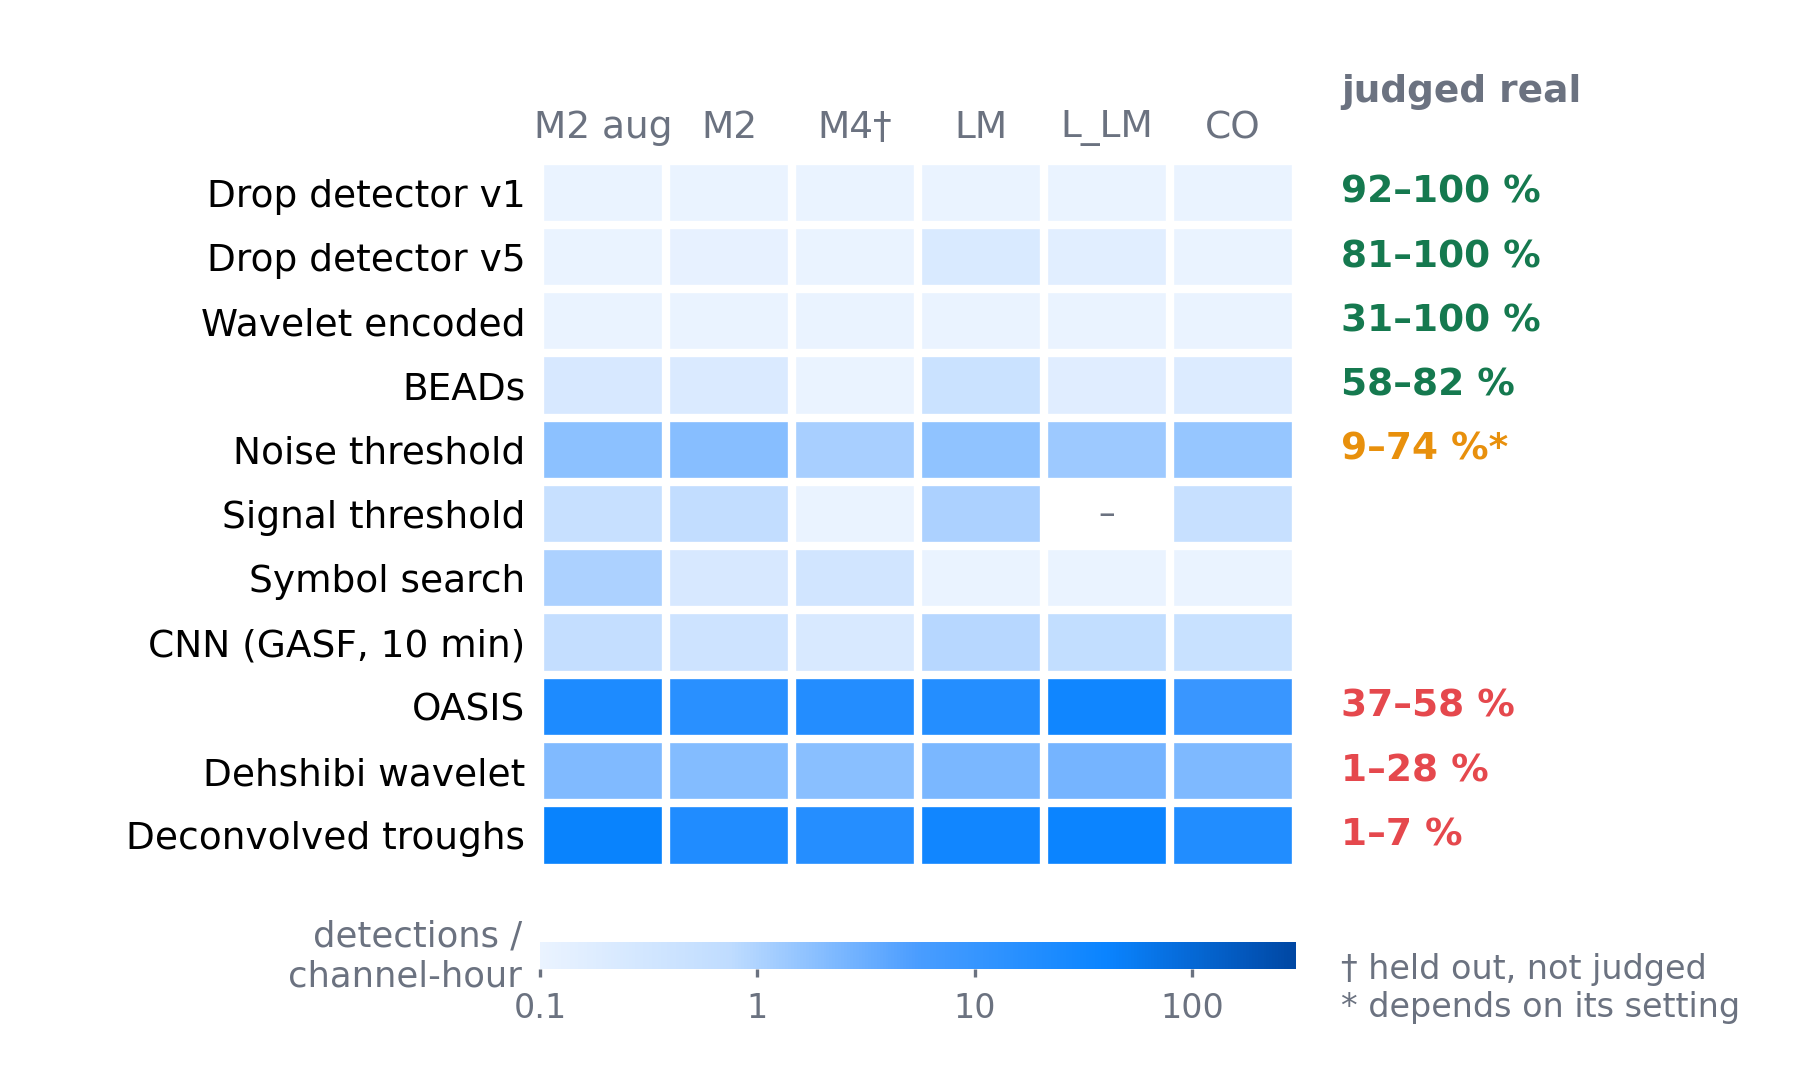
\includegraphics[width=0.95\textwidth]{poster/rq1_detectors.png}
\caption{Detection rate per channel-hour for each detector family on each recording, with the share of each family's candidates judged real across recordings. From the poster; to be redrawn without the held-out column.}
\label{fig:detectorheat}
\end{figure}

\subsection{How often candidates are real}

\begin{table}[htbp]
\caption{Estimated share of candidate events that are real, from the stratified blind samples (bootstrap 95\,\% intervals).}
\label{tab:sharereal}
\small
\begin{tabular}{lrl}
\toprule
\textbf{Recording} & \textbf{Share real} & \textbf{95\,\% interval}\\
\midrule
M2\_aug & 25\,\% & 21--28\,\%\\
LM\_fs2 & 16\,\% & 12--20\,\%\\
MJu26a (CH10, 13--16), 2\,Hz & 14\,\% & 10--19\,\%\\
M2\_concat & 13\,\% & 10--17\,\%\\
CO\_fs2 & 10\,\% & 7--13\,\%\\
\bottomrule
\end{tabular}
\end{table}

\subsection{Agreement predicts acceptance}

\begin{figure}[htbp]
\centering
\figplaceholder{6cm}{Agreement ladder: share of candidates judged real against the number of agreeing detector families (1--2, 3--4, 5--6, 7--8, 9+), one line per recording, with intervals. Data in the \texttt{estimate.json} files under \texttt{DATA/derived/candidate\_events/}. To be drawn by \texttt{scripts/thesis/}.}
\caption{The agreement ladder.}
\label{fig:ladder}
\end{figure}

\begin{instructions}
The headline is the same on every recording: 0--5\,\% of candidates are real where 1--2 families agree, and 40--63\,\%
where 9 or more agree. M2\_aug's ladder runs 4 / 6 / 22 / 54 / 59\,\% (backup deck R3, from 754 blind verdicts).

Use 40--63\,\% for the top rung. All five \texttt{estimate.json} files give it. The backup deck's 50--67\,\% does not
reproduce from any of them (\src{docs/thesis/numbers_ledger.md}).

Agreement count as a score gives AUC 0.874 on queue 25. Note for Chapter~\ref{ch:rq3}: a classifier on the events'
shape beats it.
\end{instructions}

\subsection{Choosy and loose detectors}

\begin{table}[htbp]
\caption{Share of each detector's sampled candidates judged real (``precision''), range across the five recordings, with 13--20 sampled events per detector per recording. Read as ranges, not a ranking.}
\label{tab:precision}
\small
\begin{tabular}{lll}
\toprule
\textbf{Detector family} & \textbf{Judged real} & \textbf{Note}\\
\midrule
Drop detector v1 & 92--100\,\% & choosy; about 1,000 events on M2\_aug\\
Drop detector v5 & 81--100\,\% & \\
Wavelet encoded & 86--100\,\% & 31\,\% on M2\_concat\\
BEADS (inverted) & 58--82\,\% & \\
OASIS & 37--58\,\% & 83\,\% at threshold 5, 43\,\% at threshold 3\\
Noise threshold & 9--74\,\% & depends on $k$: 74\,\% at $k=6$, 9\,\% at $k=3$\\
Dehshibi wavelet prototype & 1--28\,\% & \\
Deconvolved troughs & 1--7\,\% & \\
Matrix-profile threshold & 0\,\% & not an event detector\\
\bottomrule
\end{tabular}
\end{table}

\begin{instructions}
Add the M2\_aug-only figures from queue 25 (R3): CNN 10\,min 95\,\%, symbol search 64\,\%, signal threshold 43\,\%.
State plainly that a setting matters as much as the family: OASIS goes from 10\,k events at 83\,\% to 658\,k at
43\,\%. Each per-detector figure rests on 13--20 sampled events per recording; give Wilson intervals in the final table.
\end{instructions}

\subsection{Detectors against their surrogates}

\begin{instructions}
From \src{docs/rq_roundA_2/findings/detectors-vs-surrogates-2026-10-26.md}.

The ``255 of 552 tasks no better than the surrogate'' figure reproduces, but it covers batch 3 only (LM, CO and MJu26a CH10, 13--16, at
2\,Hz). Across all sessions it is 849 of 1,880.

The pattern runs against intuition:
\begin{itemize}
  \item the loose families (OASIS, deconvolved troughs, noise threshold) always beat their null, by 39--283$\times$;
  \item symbol search and wavelet encoded never do (0.00--0.11$\times$ the surrogate count), although their precision
        is among the highest;
  \item the drop detectors sit near 1$\times$.
\end{itemize}
The finding: with one draw per task, real-against-surrogate counts measure how much a detector responds to the
signal's spectrum, not how good its events are. This is an argument for judging precision against humans, as this
chapter does.

\textbf{The 20-draw re-run} (rangpur, 29 Oct; Table~\ref{tab:surr20}, Figure~\ref{fig:surr20}). The six most
precise variants were re-run on M2\_aug with 20 phase-randomised draws per channel. The results are in
\src{docs/rq_roundA_2/findings/surrogates20-2026-10-29.md} (ledger F8), read from the returned task records by
\src{scripts/thesis/surrogates20_readout.py}.
\begin{itemize}
  \item With 20 draws, each channel's real count is ranked against its own null. The smallest attainable $p$ is
        $1/21 \approx 0.048$, so the strongest per-channel result is ``beat all 20 draws''. Chance gives each channel
        that with probability $1/21$, which is 0.8 of 16 channels expected.
  \item Drop v1 beat all 20 draws on 16 of 16 channels, and the GADF CNN did too. The recurrence CNN and v5 at
        same-fraction 0.7 did on 14 of 16. Their binomial tails are $10^{-17}$ to $10^{-22}$, and all four pass
        Benjamini--Hochberg.
  \item Wavelet-encoded level 5 fell \emph{below} all 20 draws on 16 of 16 channels, and v1 at slope $\sigma$ 4 on 12
        of 16. Both fire more on the scrambled copies.
  \item Every pooled ratio is within 4\,\% of its 1-draw value. A single draw was not noise: how a detector stands
        against its null is a stable property of the detector.
  \item \textbf{The point for this chapter.} The two variants below their null are among the most precise in the
        blind estimate: wavelet-encoded level 5 at 0.92 and v1 at slope $\sigma$ 4 at 0.99. Beating a
        phase-randomised null and being precise are separate properties. The argument above now rests on 20 draws per
        channel, not one.
  \item \textbf{Caveat.} The binomial tails treat channels as independent, and the B4 census found a shared driver
        across packs (Chapter~\ref{ch:roundb}). Read them as approximate. The per-channel ranks are exact.
\end{itemize}
\end{instructions}

\begin{table}[htbp]
\caption{Detections on the real signal against its phase-randomised surrogate, by detector family and recording. [From the 26 Oct analysis.]}
\label{tab:detnull}
\centering
\figplaceholder{3cm}{Table to be filled from \texttt{detectors-vs-surrogates-2026-10-26.md}.}
\end{table}

\begin{table}[htbp]
\caption{Six precise variants on M2\_aug against 20 phase-randomised draws per channel (16 channels each). ``Beat all'' and ``below all'': channels whose real count lies above or below every one of its 20 draws; chance expects 0.8 of 16. Precision is from the blind queue 25 estimate.}
\label{tab:surr20}
\footnotesize
\centering
\setlength{\tabcolsep}{4pt}
\begin{tabular}{lcccccc}
\toprule
\textbf{Variant} & \textbf{Precision} & \textbf{Beat all} & \textbf{Below all} & \textbf{Ratio, 20} & \textbf{Ratio, 1} & \textbf{BH}\\
\midrule
drop v1 & 0.94 & 16/16 & 0/16 & 23.4 & 22.6 & pass\\
CNN GADF, 10 min & 0.97 & 16/16 & 0/16 & 6.5 & 6.5 & pass\\
CNN recurrence, 10 min & 0.96 & 14/16 & 1/16 & 2.7 & 2.6 & pass\\
drop v5, same fraction 0.7 & 0.81 & 14/16 & 2/16 & 2.2 & 2.2 & pass\\
drop v1, slope $\sigma$ 4 & 0.99 & 3/16 & 12/16 & 0.58 & 0.60 & --\\
wavelet-encoded, level 5 & 0.92 & 0/16 & 16/16 & 0.075 & 0.075 & --\\
\bottomrule
\end{tabular}
\end{table}

\begin{figure}[htbp]
\centering
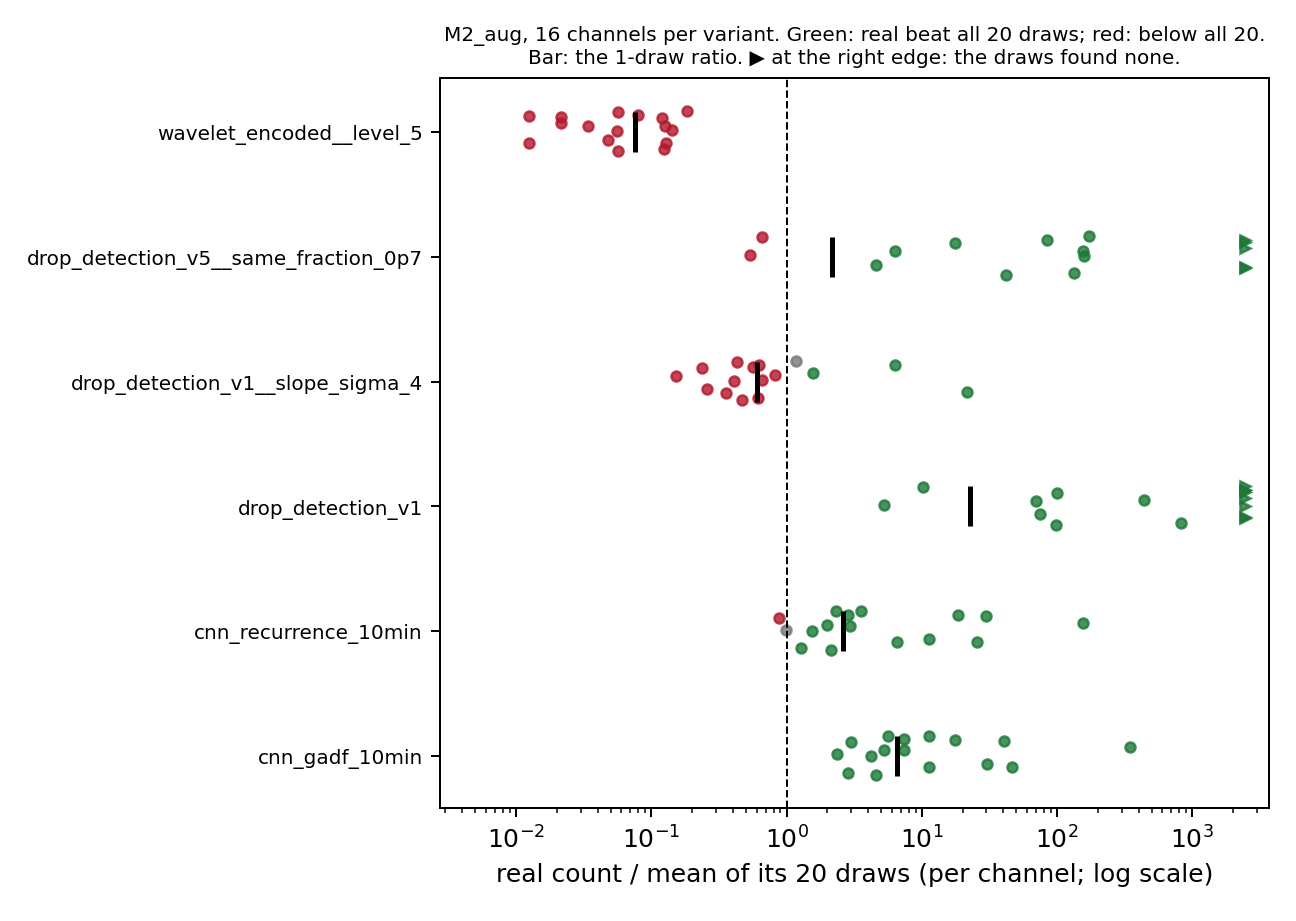
\includegraphics[width=0.9\textwidth]{data/ch06_20draw/ratio_strip.png}
\caption{Each channel's real count over the mean of its 20 draws (log scale). Green: above every draw; red: below every draw; the bar is the 1-draw ratio. A triangle at the right edge marks a channel whose 20 draws found nothing (8 for drop v1, 5 for v5).}
\label{fig:surr20}
\end{figure}

\subsection{What detectors miss}

\begin{instructions}
The miss rate, from \src{docs/rq_roundA_2/findings/miss-rate-2026-10-26.md}. This is the plan's RQ5 miss rate.
\begin{itemize}
  \item Of 2,333 manual ``interesting'' 10-minute windows on M2\_aug, no non-CNN detector touches 18 (0.8\,\%). But
        only 4.6\,\% of not-interesting windows are untouched either: coverage is high because loose detectors fire
        nearly everywhere.
  \item The useful measure is lift, a detector's touch rate on interesting windows over its rate on not-interesting
        ones: signal threshold at $-10$\,mV 21$\times$; the drop detectors about 5$\times$; OASIS 1.4$\times$; the
        1-minute CNNs 1.0$\times$; the matrix-profile threshold 0.53$\times$, anti-correlated.
  \item The CNNs are excluded from the headline, because they were very likely trained on these labels.
  \item The 18 missed windows are a re-look list in \src{docs/thesis/data/miss_rate/}.
\end{itemize} The morphology half of RQ5 (which shape classes are missed) cannot be
answered, because no verdict carries a shape tag: none of the 800 queue-25 items has a \texttt{class\_label}. Say so.
\end{instructions}

\subsection{The band-and-symbol pilot}

\begin{instructions}
Plan RQ4 as first posed: a sandbox run on M2\_aug 452--456\,h, channels CH2\_A1, CH6\_B1 and CH7\_B2.
\begin{itemize}
  \item The band chain found 75, 46 and 35 regions per layer, against nulls expecting 247.75, 125.25 and 123.35: the
        null out-finds the signal on every layer.
  \item Against drop\_detection\_v1, only the band chain 3, both 0, only the drop detector 123.
\end{itemize}
Report it as a negative pilot (\src{docs/rq_roundA/RQ4-bands-and-symbols.md}) that motivated the move to the sweep.
\end{instructions}

\section{Discussion}

\begin{instructions}
Points to argue:
\begin{itemize}
  \item Agreement among weak, independent detectors behaves like an ensemble vote, and is a good way to propose
        candidates for review. No single loose detector is.
  \item The choosy detectors (drop v1 and v5) stay right across recordings, rates (1 and 2\,Hz) and units. The loose
        ones find hundreds of thousands of events, mostly noise.
  \item Detectors that match their own surrogate measure the signal's spectrum, not its events.
\end{itemize}
Limitations:
\begin{itemize}
  \item 13--20 samples per detector;
  \item a single labeller with an 11.5\,\% miss per look;
  \item recall is not measurable, because no complete human reference exists;
  \item the one-draw surrogate;
  \item precision is precision against your judgement, not against a biological truth.
\end{itemize}
Tie back to the literature: no published fungal detector reports any of these numbers.
\end{instructions}
